\chapter[SCP-122 再无怪物]{
    SCP-122 No More Monsters\\
    SCP-122 再无怪物
}

\label{chap:SCP-122}

\begin{figure}[H]
    \centering
    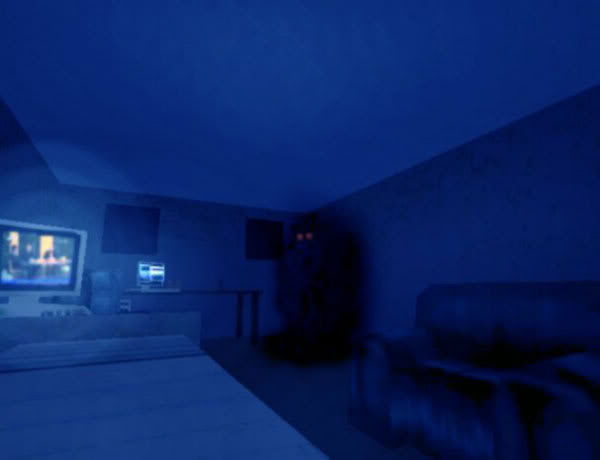
\includegraphics[width=0.5\linewidth]{images/SCP.122.jpg}
    \caption*{SCP-122-1的个体}
\end{figure}

\bb{项目编号:}SCP-122

\bb{项目等级:}Keter

\bb{特殊收容措施:}SCP-122收容于一间带有单一电源输出的标准收容间中。收容区域500m以内严禁设置住宿设施。严禁SCP-122于任何时刻处于无电力状态下。数个备用电力系统应接受定期维护与检修。当出现SCP-122-1显现的状况下,35名之前奉命处置该对象的基金会人员将被调离收容区域。一旦对象表现出敌对性,将采用程序-99-Renmar进行应对。

为保证程序-99-Renmar执行,所有人员应于收容间内部以及周边的预定地点就位,以防止收容突破的发生。两名基金会人员负责操作便携式发电机,对执行程序-99-Renmar的装备保持电力供应。三名基金会人员需持有作为\hyperref[chap:SCP-1837]{SCP-1837}副产品所产生的化学刺激性物品,已证明该物质对SCP-122-1的个体具有抑制作用。

当SCP-122-1的所有个体被削减至能够保证入口安全之时,五名基金会人员将进入收容间,并使用携带的延长电线通过与发电机相连恢复SCP-122的电力供应。鉴于SCP-122的性质,以上五名人员在进入其收容间将被判定为不可痊愈。

剩余人员则作为后备,将用以代替无法继续工作的员工。

\bb{描述:}SCP-122的外形是一盏设计成流星特效的儿童用小夜灯。当其处用电力供应状态下时,SCP-122所释放出光照度为14-20勒克斯。SCP-122组件的表面以及灯具内部未发现其制造商的相关信息。

当SCP-122处于无电力状态下时,SCP-122将会对其周边500m范围内的人员产生影响。当对象处于快速眼动睡眠状态时,将会陷入昏迷状态中直到SCP-122重新恢复供电。当处于昏迷过程中时,对象附近将会出现人形身影。此类身影在此被定义为SCP-122-1。

SCP-122-1的个体表现出了具有智力以及感性的行为,且物理性能约等于受影响个体。它们会试图使尽可能多地寻找人类个体并使之暴露于SCP-122之下。受影响的人类个体越多,SCP-122的作用半径则越大,实验中已确认的最大半径超过了2.7公里。SCP-122-1的个体将试图在SCP-122的作用范围内收集所有的助眠物品,并将其应用在受影响的个体上。这些物品包括:

\begin{itemize}
\item 安眠药物
\item 用于治疗失眠症的传统药物
\item 枕头,毯子,床垫,床架
\item 媒体手段譬如摇篮曲
\end{itemize}

当SCP-122处于供电状态下时,它将对其作用半径内所有的对象的睡眠模式产生影响。如果一名处于SCP-122作用半径内的快速眼动睡眠对象苏醒,该对象将会表现出失眠的症状,且抱怨道做了一个非同寻常的梦。\dd{这些梦境被发现会对对象造成轻微的心理层面上的干扰,且所有人员都应接受每周一次的心理评估。}参见事件122-1。

安插在当地的特工在收到了数份关于SCP-122-1显现的报告后,SCP-122于████年██月██日被发现于██████儿童医院。在对该区域进行调查时发现,该建筑内所有对象均已受SCP-122影响。回收文档中记录道SCP-122是由一名病人在得到许可后带入的。然而,未发现该病人的相关信息。特工们使用移动电源对SCP-122进行压制后将其移送至Site-19。

\bb{附录 122-B:}SCP-122在事件122-1之后重新分级为Keter。对象已转移至武装收容区-02(Armed Reliquary Containment Area-02)。

\bb{事件122-1:}████年██月██日,11例SCP-122-1个体发生收容突破,导致█名基金会人员死亡以及██人受伤。在进行了二次收容后,SCP-122的收容措施被重新审查。在调查过程中,安全录像显示数名维护人员对SCP-122的收容安全锁进行了破坏。直到释放了SCP-122后才进入睡眠状态。受影响的对象已经手了A级记忆消除程序,收容措施已经修订。已申请升级为Keter。
